\begin{figure}[h!]
    \centering
    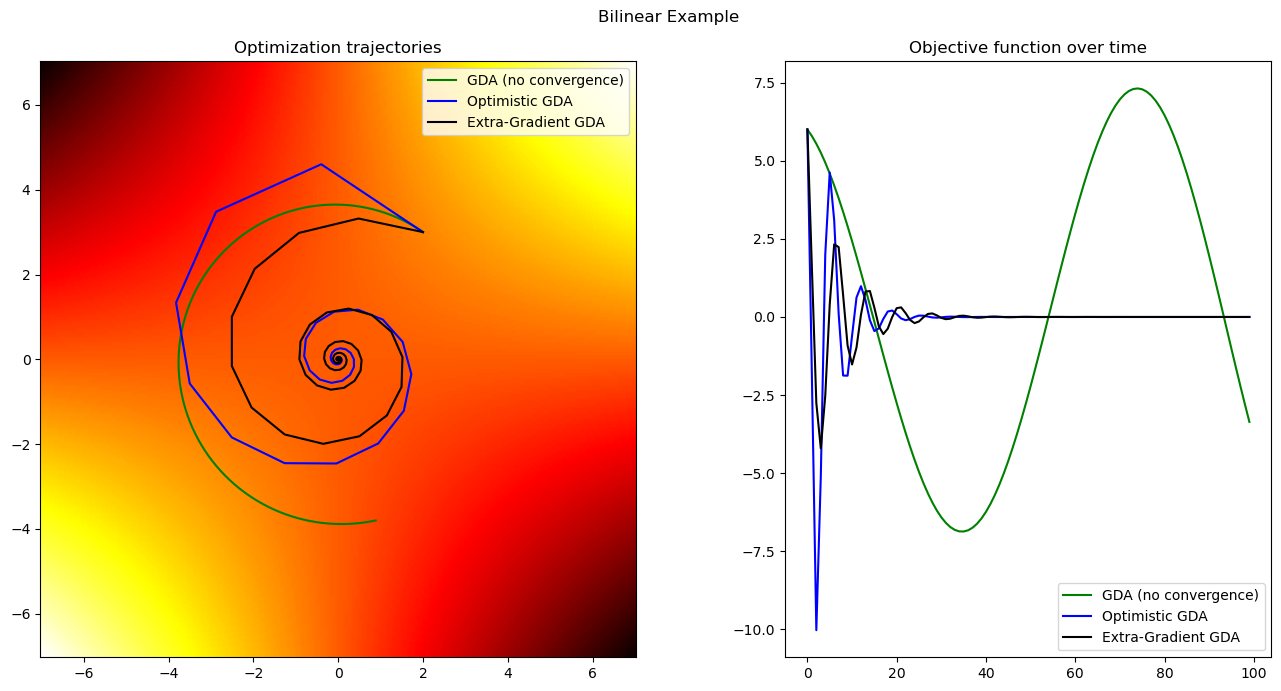
\includegraphics[width=\textwidth]{figures/bilinear_opt.png}
    \caption{Iterations of three optimization methods (Gradient Descent-Ascent, Optimistic Gradient and Extra Gradient methods) on an unconstrained bilinear saddle-point optimization problem.}
\end{figure}

In the following section, we introduce, discuss and analyze algorithms for solving \textit{saddle-point} problems of the form; 
\begin{align*}
    \min_{\bm{x} \in X} \max_{\bm{y} \in Y} f(\bm{x},\bm{y}).
\end{align*}
Where $f:X \times Y \rightarrow \mathbb{R}$ is some scalar function for which we want to find a \textit{saddle point}, i.e. a point $(\bm{x}^*,\bm{y}^*)\in X \times Y$, s.t.
\begin{align*}
    f(\bm{x}^*,\bm{y}) \leq  f(\bm{x}^*,\bm{y}^*) \leq f(\bm{x},\bm{y}^*),
\end{align*}
i.e. in plain english "\textit{$(\bm{x}^*,\bm{y}^*)$ is a minimizer in $\bm{x}$ and a maximizer in $\bm{y}$}". Such problems which will prove especially relevant in our study of inverse reinforcement learning. \\

\subsection{Preliminaries}

\begin{definition}
    (\textbf{Lipschitz-continuous function}) A function $f: \textbf{dom}(f) \rightarrow \mathbb{R}^m$ is $B$-Lipschitz if for any $\bm{x},\bm{y} \in \textbf{dom}(f)$, there exists $B \in \mathbb{R}_+$\:
    \[
      \|f(\bm{x})-f(\bm{y})\| \leq B \| \bm{x} - \bm{y} \|.
    \]
\end{definition}


\begin{definition}
    (\textbf{Smooth function}) A function $f : \textbf{dom}(f) \rightarrow \mathbb{R}$ is called $L$-smooth if it has $L$-Lipschitz continuous gradients, i.e. if for any $\bm{x},\bm{y} \in \textbf{dom}(f)$, there exists $L \in \mathbb{R}_+$:
    \[
      \|\nabla f(\bm{x}) -\nabla f(\bm{y})\| \leq L \| \bm{x} - \bm{y} \|.
    \]
\end{definition}

\begin{definition}
    (\textbf{Convex set}) A set $C \subseteq \mathbb{R}^d$ is convex if for any two points $\bm{x},\bm{y} \in \mathbb{R}^d$, the connecting line segment is contained in $C$, i.e. $\forall \lambda, \lambda \in [0,1]$:
    \[  \lambda \bm{x} + (1-\lambda) \bm{y} \in C.\]
\end{definition}

\begin{definition}
    (\textbf{Convex function}) A function $f : \textbf{dom}(f) \rightarrow \mathbb{R}$ is called convex on $\textbf{dom}(f)$ if 
    \begin{enumerate}
        \item $\textbf{dom}(f)$ is convex,
        \item for all $\bm{x}, \bm{y} \in  \textbf{dom}(f)$ and $\lambda \in [0,1]$ we have:
        \[  f(\lambda \bm{x} + (1-\lambda) \bm{y}) \leq \lambda f(\bm{x}) + (1-\lambda) f(\bm{y}). \]
    \end{enumerate}
\end{definition}

\begin{definition}
    (\textbf{Concave function}) A function $f : \textbf{dom}(f) \rightarrow \mathbb{R}$ is called concave on $\textbf{dom}(f)$ if the function $g : \textbf{dom}(f) \rightarrow \mathbb{R}$ defined as $g(x)= -f(x)$ is convex on $\textbf{dom}(f)$.
\end{definition}

\begin{definition}
    \label{def:saddle_point}
    (\textbf{Saddle point}) The point $(\bm{x}^*,\bm{y}^*)\in X \times Y$  is a saddle point of the function $f:X,Y \rightarrow \mathbb{R}$ if for any $\bm{x} \in X$ and $\bm{y} \in Y$ we have:
     \[ f(\bm{x}^*,\bm{y}) \leq f(\bm{x}^*,\bm{y}^*) \leq f(\bm{x},\bm{y}^*). \]
\end{definition}

\begin{definition}
    \label{def:saddle_point_problem}
    (\textbf{Saddle-Point Problem}) Consider $f:X,Y \rightarrow \mathbb{R}$ a continuously differentiable scalar function on  convex domains $X \subseteq \mathbb{R}^n$ and $Y \subseteq \mathbb{R}^m$. For convenience use notation $Z = X\times Y$ and $z=(x,y)$. We call the optimization problem below:
    \begin{align*}
        \min_{\bm{x} \in X} \max_{\bm{y} \in Y} f(\bm{x},\bm{y}).
    \end{align*}
    a saddle point problem. The solution set $\mathcal{Z}$ defined as:
    \begin{align*}
        \mathcal{Z} := \Big\lbrace (x^*,y^*) \in X \times Y  
        \Big |  f(\bm{x}^*,\bm{y}) \leq f(\bm{x}^*,\bm{y}^*) \leq f(\bm{x},\bm{y}^*), ~ \forall x \in X, ~y \in Y
        \Big\rbrace
    \end{align*}
    is the set of all saddle points (see def \ref{def:saddle_point}) of the function $f$. Such a problem can be constrained ($X \subset \mathbb{R}^n$ and $Y \subset \mathbb{R}^m$) or unconstrained  ($X = \mathbb{R}^n$, $Y = \mathbb{R}^m$).
\end{definition}


\begin{definition}
    (\textbf{Convex-Concave Problem}) Consider a saddle point problem (see def \ref{def:saddle_point_problem}), defined by $f:X,Y \rightarrow \mathbb{R}$ a continuously differentiable scalar function on convex domains $X \subseteq \mathbb{R}^n$ and $Y \subseteq \mathbb{R}^m$. We call the problem a convex-concave problem if $f$ is convex in $x$ and concave in $y$.
\end{definition}

\begin{proposition}
    In general:
    \begin{align*}
        \max_{\bm{x} \in X} \min_{\bm{y} \in Y} f(\bm{x},\bm{y}) \leq \min_{\bm{y} \in Y} \max_{\bm{x} \in X} f(\bm{x},\bm{y}).
    \end{align*}
\end{proposition}
\begin{proof}
    Let $\tilde{\bm{x}} = \arg \max_{\bm{y} \in Y} \min_{\bm{x} \in X} f(x,y)$, $\tilde{\bm{y}} = \arg \max_{\bm{y} \in Y} \min_{\bm{x} \in X} f(x,y)$,
\end{proof}

\begin{theorem}
    (\textbf{Sion's Minimax Theorem} \cite{sion_general_1958}) If $X$ and $Y$ are convex compact sets, and if $f:X \times Y \rightarrow \mathbb{R}$ is convex concave, then: 
    \begin{align*}
        \max_{\bm{x} \in X} \min_{\bm{y} \in Y} f(\bm{x},\bm{y}) = \min_{\bm{y} \in Y} \max_{\bm{x} \in X} f(\bm{x},\bm{y}).
    \end{align*}
\end{theorem}

\begin{definition}
    (\textbf{Projection Operator}) given some convex set $S \subseteq \mathbb{R}^n$ as well a point $\bm{x} \in \mathbb{R}^n$, we define the projection $\bm{p}$ of $\bm{x}$ onto $S$ as:
    \begin{align*}
        \bm{p} = \arg \min_{\bm{y} \in S} \| \bm{x} - \bm{y} \|,
    \end{align*}
    which we often simply denote as the output of the projection operator associated with the set S: 
    \begin{align*}
        \Pi_S(\bm{x}) := \arg \min_{\bm{y} \in S} \| \bm{x} - \bm{y} \|.
    \end{align*}
    When the norm used is the Euclidian norm (or $L_2$ norm), we call this operation the Euclidian Projection.
\end{definition}

\begin{definition}
    (\textbf{Duality Gap}) We define the duality gap as a way of characterizing the sub-optimality of a point. Given some point $\tilde{\bm{z}}=(\tilde{\bm{x}},\tilde{\bm{y}})\in Z$, its duality gap is given by:
    \begin{align*}
        \text{Duality Gap}(\tilde{\bm{z}}) := \max_{\bm{y} \in Y} f(\tilde{\bm{x}},\bm{y}) - \min_{\bm{x} \in X} f(\bm{x},\tilde{\bm{y}})
    \end{align*}
\end{definition}


\subsection{Gradient Descent Ascent} \label{sec:GDA}

The most simple algorithm is the natural extension of gradient descent/ascent to the saddle point problem. In the following section, we define the gradient descent-ascent (GDA) algorithm, analyze it and discuss it's performance and limitations. Note that we specifically analyze \textit{projected} gradient descent-ascent, as results for projected GDA trivially generalize to unconstrained GDA and the projected setting will be useful for our applications in inverse reinforcement learning.


\begin{algorithm}[H]
    \label{alg:projGDA}
    \SetAlgoLined
    \caption{(Projected) Gradient Descent Ascent}
    Set the learning rate $\eta >0$ \\
    Initialize the algorithm at some point $(\bm{x}_0,\bm{y}_0)$  \\
    \ForEach{iteration $k = 0,2,...,K-1$}{
        $\bm{x}_{k+1} \leftarrow \Pi_X \big(\bm{x}_k - \eta \nabla_x f(x_k,y_k)\big)$ \\
        $\bm{y}_{k+1} \leftarrow \Pi_Y \big(\bm{y}_k + \eta \nabla_y f(x_k,y_k) \big)$ \\
    }
    return $(\bm{x}_N,\bm{y}_N)$
\end{algorithm}

\begin{proposition}
    \label{prop:proj_gda_convex_concave}
    (\textbf{$O(\frac{1}{\sqrt{K}})$ convergence rate}) For $B$-Lipschitz convex concave functions $f:X,Y \rightarrow \mathbb{R}$, defined on two convex domains $X$ and $Y$ with bounded diameter $D=\max \lbrace  \text{diam}(X), \text{diam}(Y) \rbrace$, after $K$ steps, projected gradient descent-ascent (alg \ref{alg:projGDA}) with learning rate $\eta_k = \frac{D}{\sqrt{2k}B}$ has gives an average point for which the duality gap is bounded by:
    \[
        \text{Duality Gap}(\bar{\bm{z}}_K) \leq \frac{4 D B}{\sqrt{K}},
    \]
    where $\bar{\bm{z}}_K = \frac{1}{K} \sum_{k = 1...K} (\bm{x}_k,\bm{y}_k)$.
\end{proposition}
\begin{proof}
    (of proposition \ref{prop:proj_gda_convex_concave}) Given a fixed-point $\bm{z}^*=(\bm{x}^*,\bm{y}^*)$, using the projected gradient update on $\bm{x}$ we get:
    \begin{align*}
        \| \bm{x}_{k+1}-\bm{x}^* \|^2 &= \| \Pi_X(\bm{x}_{k}-\eta_k \nabla_x f(\bm{x}_k,\bm{y}_k) ) - \Pi(\bm{x}^*) \|^2 && \text{since $\bm{x}^*\in X$} \\
        &\leq \| \bm{x}_{k}-\eta_k \nabla_x f(\bm{x}_k,\bm{y}_k) - \bm{x}^* \|^2 && \text{projections are non-expansive} \\
        & = \| \bm{x}_k - \bm{x}^* \|^2 + \eta_k^2 \| \nabla_x f(\bm{x}_k,\bm{y}_k)\|^2  \\ & ~ ~ - 2 \eta_K \langle  \bm{x}_k - \bm{x}^*,  \nabla_x f(\bm{x}_k,\bm{y}_k) \rangle \\
        & \leq \| \bm{x}_k - \bm{x}^* \|^2 + \eta_k^2 B^2 && \text{since $f$ is $B$-Lipschitz} \\ & ~ ~ - 2  \eta_K [f(\bm{x}_k,\bm{y}_k)-f(\bm{x}^*,\bm{y}_k)] && \text{by convexity of $f$}\\
    \end{align*}
    And thus:
    \begin{align*}
        \Rightarrow ~~~ f(\bm{x}_k,\bm{y}_k)-f(\bm{x}^*,\bm{y}_k) \leq \frac{  \| \bm{x}_k - \bm{x}^* \|^2 - \| \bm{x}_{k+1}-\bm{x}^* \|^2
        }{2 \eta_K
        } + \frac{\eta_K}{2} B^2. \tag{a}
    \end{align*}
    Similarly using the projected gradient update on $\bm{y}$ we have:
    \begin{align*}
        \| \bm{y}_{k+1}-\bm{y}^* \|^2 &\leq \| \bm{y}_k - \bm{y}^* \|^2 + \eta_k^2 \| \nabla_y f(\bm{x}_k,\bm{y}_k)\|^2 \\ &  + 2 \eta_K \langle  \bm{y}_k - \bm{y}^*,  \nabla_y f(\bm{x}_k,\bm{y}_k) \rangle \\
        & \leq \| \bm{y}_k - \bm{y}^* \|^2 + \eta_k^2 B^2 && \text{since $f$ is $B$-Lipschitz} \\ & ~ ~ - 2  \eta_K [f(\bm{x}_k,\bm{y}_k)-f(\bm{x}_k,\bm{y}^*)] && \text{by concavity of $f$}\\
    \end{align*}
    And thus:
    \begin{align*}
        \Rightarrow ~~~ f(\bm{x}_k,\bm{y}^*) - f(\bm{x}_k,\bm{y}_k) \leq \frac{  \| \bm{y}_k - \bm{y}^* \|^2 - \| \bm{y}_{k+1}-\bm{y}^* \|^2
        }{2 \eta_K
        } + \frac{\eta_K}{2} B^2. \tag{b}
    \end{align*}
    Adding ($a$) and ($b$) together we get:
    \begin{align*}
        f(\bm{x}_k,\bm{y}_k)-f(\bm{x}^*,\bm{y}_k) + f(\bm{x}_k,\bm{y}^*) - f(\bm{x}_k,\bm{y}_k) = f(\bm{x}_k,\bm{y}^*) -f(\bm{x}^*,\bm{y}_k) \\
        \leq 
        \frac{  \| \bm{x}_k - \bm{x}^* \|^2 - \| \bm{x}_{k+1}-\bm{x}^* \|^2
        }{2 \eta_K} +
        \frac{ \| \bm{y}_k - \bm{y}^* \|^2 - \| \bm{y}_{k+1}-\bm{y}^* \|^2
        }{2 \eta_K} +
        \eta_K B^2. \tag{c}
    \end{align*}
    Summing up over all optimization steps we have:
    \begin{align*}
        \sum_{k=1...K} f(\bm{x}_k,\bm{y}^*) -f(\bm{x}^*,\bm{y}_k) \\
        \leq \sum_{k=1...K} \Bigg[
        \frac{  \| \bm{x}_k - \bm{x}^* \|^2 - \| \bm{x}_{k+1}-\bm{x}^* \|^2
        }{2 \eta_K} \Bigg] \\+ \sum_{k=1...K} \Bigg[
        \frac{ \| \bm{y}_k - \bm{y}^* \|^2 - \| \bm{y}_{k+1}-\bm{y}^* \|^2
        }{2 \eta_K}  \Bigg]  +
        B^2 \sum_{k=1...K}\eta_K. \tag{d}
    \end{align*}
    Observing that the terms in the sum telescope we have:
    \begin{align*}
        \sum_{k=1...K} \Bigg[ \frac{  \| \bm{x}_k - \bm{x}^* \|^2 - \| \bm{x}_{k+1}-\bm{x}^* \|^2
        }{2 \eta_K} \Bigg]  \leq \frac{D^2}{2 \eta_K} \\
        \sum_{k=1...K} \Bigg[
        \frac{ \| \bm{y}_k - \bm{y}^* \|^2 - \| \bm{y}_{k+1}-\bm{y}^* \|^2
        }{2 \eta_K}  \Bigg] \leq \frac{D^2}{2 \eta_K}.
    \end{align*}
    Which once plugged into ($d$) give:
    \begin{align*}
        \sum_{k=1...K} f(\bm{x}_k,\bm{y}^*) -f(\bm{x}^*,\bm{y}_k) \leq 
        \frac{D^2}{\eta_K} + B^2 \sum_{k=1...K}\eta_k = \frac{D^2 \sqrt{K}}{\eta} + B^2 \eta \sum_{k=1...K}\frac{1}{\sqrt{k}} \\
        \leq  \frac{D^2 \sqrt{K}}{\eta} +2 B^2 \eta \sqrt{K}.
    \end{align*}
    Thus we have:
    \begin{align*}
        \frac{1}{K} \Big[ \sum_{k=1...K} f(\bm{x}_k,\bm{y}^*) -f(\bm{x}^*,\bm{y}_k)  \Big] \leq \frac{D^2 }{ \eta \sqrt{K}} +  2 B^2 \eta \frac{1}{\sqrt{K}}  \\
        \text{(Optimizing $\eta$) } = \frac{4DB}{\sqrt{K}} 
    \end{align*}
\end{proof}

% \subsection{Proximal Point Method}
% {
% \color{red}
% TODO : maybe analyze it to get an idea of why we try to approximate it with EG.
% }
\subsection{Extra-Gradient Descent Ascent}
\label{sec:extra_grad}
\begin{figure}[h!]
    \centering
    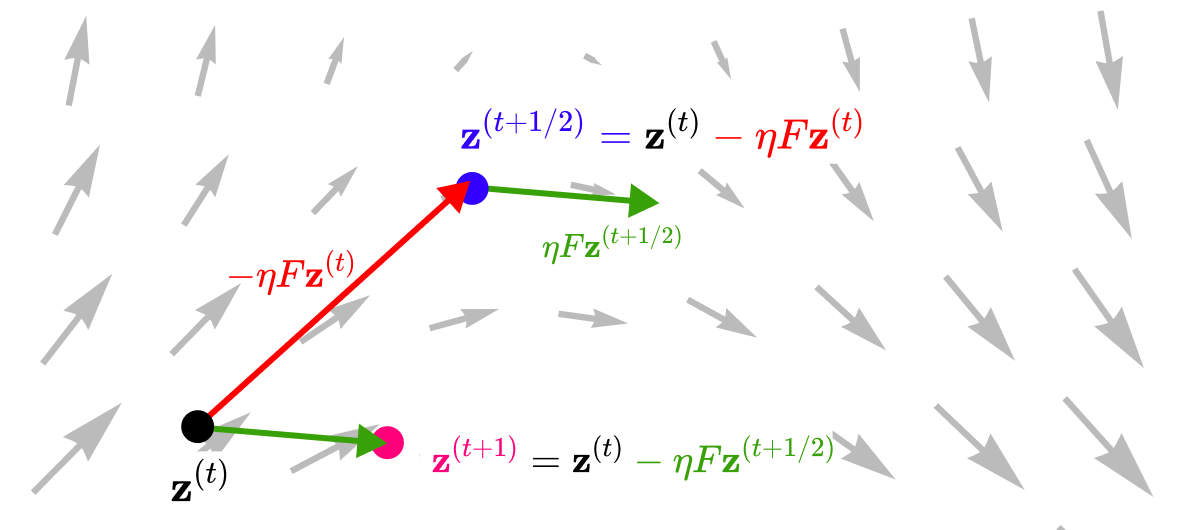
\includegraphics[width=0.8\textwidth]{figures/Extra_Gradient.png}
    \caption{An illustration of an extra-gradient step.}
\end{figure}
Next, we consider the Extra-Gradient Descent Ascent method (EG), which provides an approximation of the \textit{implicit} proximal point method and has better performance compared to the naïve GDA approach, specifically:
\begin{enumerate}
    \item a better convergence rate on general convex-concave programs ($O(\frac{1}{K})$ instead of $O(\frac{1}{\sqrt{K}})$)
    \item last iterate convergence for all convex-concave functions, including for bilinear functions (which isn't true for naïve GDA).
\end{enumerate}

As in the naïve GDA case, we choose to analyze \textit{projected} EG, because this will prove useful to solve the IRL problems we are concerned about.

\begin{algorithm}[H]
    \label{alg:projEG}
    \SetAlgoLined
    \caption{(Projected) Extra-Gradient Descent Ascent}
    Set the learning rate $\eta >0$ \\
    Initialize the algorithm at some point $(\bm{x}_0,\bm{y}_0)$  \\
    \ForEach{iteration $k = 0,2,...,K-1$}{
        $\bm{x}_{k+1/2} \leftarrow \Pi_X \big(\bm{x}_k - \eta \nabla_x f(\bm{x}_k,\bm{y}_k)\big)$ \\
        $\bm{y}_{k+1/2} \leftarrow \Pi_Y \big(\bm{y}_k + \eta \nabla_y f(\bm{x}_k,\bm{y}_k) \big)$ \\
        $\bm{x}_{k+1} \leftarrow \Pi_X \big(\bm{x}_k - \eta \nabla_x f(\bm{x}_{k+1/2},\bm{y}_{k+1/2})\big)$ \\
        $\bm{y}_{k+1} \leftarrow \Pi_Y \big(\bm{y}_k + \eta \nabla_y f(\bm{x}_{k+1/2},\bm{y}_{k+1/2}) \big)$ \\
    }
    return $(\bm{x}_K,\bm{y}_K)$
\end{algorithm}

In order to make the computations a bit lighter, we will use the following notation, let $F$ denote the flow (the direction of gradients ascending and descending) of GDA/EG:
\begin{align*}
    F(\bm{z}) = \begin{bmatrix}
        \nabla_{\bm{x}} f(\bm{x},\bm{y}) \\
        -\nabla_{\bm{y}} f(\bm{x},\bm{y}).
    \end{bmatrix}
\end{align*}
We also define a single the feasible set $S:=\{ \bm{z}=(\bm{x},\bm{y}); \bm{x} \in X, \bm{y} \in Y\}$, and it's associated projection operator $\Pi_S(\bm{z}) = [\Pi_X(\bm{x}),\Pi_Y(\bm{y})]^T$.
In this setting we can express the EG updates, in a much more concise form as:
\begin{align*}
    \bm{z}_{k+1/2} = \Pi_S(\bm{z}_{k}-\eta F(\bm{z}_k)),\\
    \bm{z}_{k+1} = \Pi_S(\bm{z}_{k}-\eta F(\bm{z}_{k+1/2})).
\end{align*}

Given a fixed point $\bm{z}^*$, and using the first order characterization of optimality we have that $\forall (\bm{x},\bm{y}) \in X \times Y$:
\begin{equation*}
    \begin{aligned}
        \langle \nabla_x f(\bm{x}^*,\bm{y}),\bm{x}-\bm{x}^* \rangle \geq 0,\\
        \langle -\nabla_y f(\bm{x},\bm{y}^*),\bm{y}-\bm{y}^* \rangle \geq 0.
    \end{aligned}
\end{equation*}
which can be expressed more concisely as:
\begin{align*}
    \Bigg \langle  \begin{bmatrix}
        \nabla_x f(\bm{x}^*,\bm{y}) \\
        -\nabla_y f(\bm{x},\bm{y}^*)
    \end{bmatrix} ,
    \begin{bmatrix}
        \bm{x} \\ 
        \bm{x}^* 
    \end{bmatrix}
    -
    \begin{bmatrix}
        \bm{y}^* \\
        \bm{y}^*
    \end{bmatrix}
    \Bigg \rangle \geq 0 \Rightarrow \langle F(\bm{z}^*),\bm{z}-\bm{z}^* \rangle \geq 0.
\end{align*}
Observe that for $\nabla f$ $\mu$-Lipschitz, $F$ is a $2\mu$-Lipschitz operator.

\begin{proposition}
    \label{prop:proj_eg_smooth_convex_concave}
    For $\mu$-smooth convex-concave functions, where $X$ and $Y$ have max diameter $D$, expected gradient with $\eta_k = \frac{1}{2\mu}$ gives the following duality gap for the expected steps:
    the duality gap is bounded by:
    \[
        \text{Duality Gap}(\bar{\bm{z}}_K) \leq \frac{2 D^2 \mu}{K},
    \]
    where $\bar{\bm{z}}_K = \frac{1}{K} \sum_{k = 1...K} (\bm{x}_k,\bm{y}_k)$.
\end{proposition}


\begin{proof}
For some $\bm{x} \in X$, $\bm{y} \in Y$, we have:
\begin{align*}
    f(\bm{x}_{k+1/2},\bm{y}) - f(\bm{x},\bm{y}_{k+1/2}) \\
    = f(\bm{x}_{k+1/2},\bm{y}) \overbrace{- f(\bm{x}_{k+1/2},\bm{y}_{k+1/2}) + f(\bm{x}_{k+1/2},\bm{y}_{k+1/2})}^{=0}  - f(\bm{x},\bm{y}_{k+1/2}) \\
    \text{(by convexity/concavity)} \\
    \leq \langle \nabla_{\bm{y}} f(\bm{x}_{k+1/2},\bm{y}_{k+1/2}),\bm{y}- \bm{y}_{k+1/2} \rangle +
    \langle \nabla_{\bm{x}} f(\bm{x}_{k+1/2},\bm{y}_{k+1/2}), \bm{x}_{k+1/2} - \bm{x}\rangle  \\
    = 
    \Bigg \langle  
    \begin{bmatrix}
        \nabla_x f(\bm{x}_{k+1/2},\bm{y}_{k+1/2}) \\
        -\nabla_y f(\bm{x}_{k+1/2},\bm{y}_{k+1/2})
    \end{bmatrix} ,
    \begin{bmatrix}
        \bm{x}_{k+1/2} -\bm{x} \\ 
        \bm{y}_{k+1/2} - \bm{y}
    \end{bmatrix}
    \Bigg \rangle \\
    \Rightarrow f(\bm{x}_{k+1/2},\bm{y}) - f(\bm{x},\bm{y}_{k+1/2}) \leq 
    \langle F(\bm{z}_{k+1/2}), \bm{z}_{k+1/2} -\bm{z} \rangle.
\end{align*}
This provides us with a way to bound $\langle F(\bm{z}_{k+1/2}), \bm{z}_{k+1/2} -\bm{z} \rangle$ and thus the duality gap, by finding some upper-bound for the right-hand side of the equation, $\langle F(\bm{z}_{k+1/2}), \bm{z}_{k+1/2} -\bm{z} \rangle$, which is what we will do next.
\begin{align*}
    \langle F(\bm{z}_{k+1/2}), \bm{z}_{k+1/2} -\bm{z} \rangle
    = \Bigg \langle\frac{\bm{z}_k-\tilde{\bm{z}}_{k+1}}{\eta}, \bm{z}_{k+1/2} -\bm{z} \Bigg\rangle \\ \text{(From the upddates, the tilde means before projection.)} \\
    = \Bigg \langle\frac{\bm{z}_k-\tilde{\bm{z}}_{k+1}}{\eta}, \bm{z}_{k+1/2} - \bm{z}_{k+1} \Bigg\rangle +
    \Bigg \langle\frac{\bm{z}_k-\tilde{\bm{z}}_{k+1}}{\eta}, \bm{z}_{k+1} -\bm{z} \Bigg\rangle \\ \text{Adding $0=\bm{z}_{k+1}-\textbf{z}_{k+1}$} \\
    \leq \Bigg \langle\frac{\bm{z}_k-\tilde{\bm{z}}_{k+1}}{\eta}, \bm{z}_{k+1/2} -\bm{z}_{k+1} \Bigg\rangle +
    \Bigg \langle\frac{\bm{z}_k-{\bm{z}}_{k+1}}{\eta}, \bm{z}_{k+1} -\bm{z} \Bigg\rangle \\  
    \text{(Using that }
    \langle \tilde{\bm{z}}_{k+1} - {\bm{z}}_{k+1}, \bm{z} -\bm{z}_{k+1} \rangle \Rightarrow 
    \langle - \tilde{\bm{z}}_{k+1} , \bm{z} -\bm{z}_{k+1} \rangle \leq - {\bm{z}}_{k+1}, \bm{z} -\bm{z}_{k+1} \rangle\\
    \text{from the properties of the projection operator.)} \\
    = \Bigg \langle\frac{\bm{z}_k-\tilde{\bm{z}}_{k+1/2}}{\eta}, \bm{z}_{k+1/2} -\bm{z}_{k+1} \Bigg\rangle +
    \Bigg \langle\frac{\tilde{\bm{z}}_{k+1/2}-\tilde{\bm{z}}_{k+1}}{\eta}, \bm{z}_{k+1/2} -\bm{z}_{k+1} \Bigg\rangle \\+ 
    \Bigg \langle\frac{\bm{z}_k-{\bm{z}}_{k+1}}{\eta}, \bm{z}_{k+1} -\bm{z} \Bigg\rangle \\  
    \text{Adding $0=\tilde{\bm{z}}_{k+1/2}-\tilde{\bm{z}}_{k+1/2}$} \\
\end{align*}
\begin{align*}
    = \Bigg \langle\frac{\bm{z}_k-{\bm{z}}_{k+1/2}}{\eta}, \bm{z}_{k+1/2} -\bm{z}_{k+1} \Bigg\rangle +
    \Bigg \langle\frac{\tilde{\bm{z}}_{k+1/2}-\tilde{\bm{z}}_{k+1}}{\eta}, \bm{z}_{k+1/2} -\bm{z}_{k+1} \Bigg\rangle \\+ 
    \Bigg \langle\frac{\bm{z}_k-{\bm{z}}_{k+1}}{\eta}, \bm{z}_{k+1} -\bm{z} \Bigg\rangle \\  
    \text{(Using that }
    \langle \tilde{\bm{z}}_{k+1/2} - {\bm{z}}_{k+1/2}, \bm{z} -\bm{z}_{k+1/2} \rangle \\\Rightarrow 
    \langle - \tilde{\bm{z}}_{k+1/2} , \bm{z}_{k+1/2} -\bm{z} \rangle \leq - {\bm{z}}_{k+1/2}, \bm{z}_{k+1} -\bm{z} \rangle\\
    \text{from the properties of the projection operator.)} \\
\end{align*}
We thus have an expression made up of three terms:
\begin{align*}
    \langle F(\bm{z}_{k+1/2}), \bm{z}_{k+1/2} -\bm{z} \rangle \leq \Bigg \langle\frac{\bm{z}_k-{\bm{z}}_{k+1/2}}{\eta}, \bm{z}_{k+1/2} -\bm{z}_{k+1} \Bigg\rangle + \\
    \Bigg \langle\frac{\tilde{\bm{z}}_{k+1/2}-\tilde{\bm{z}}_{k+1}}{\eta}, \bm{z}_{k+1/2} -\bm{z}_{k+1} \Bigg\rangle + 
    \Bigg \langle\frac{\bm{z}_k-{\bm{z}}_{k+1}}{\eta}, \bm{z}_{k+1} -\bm{z} \Bigg\rangle \\
    \Rightarrow \eta \langle F(\bm{z}_{k+1/2}), \bm{z}_{k+1/2} -\bm{z} \rangle \leq
    \overbrace{\langle \bm{z}_k-{\bm{z}}_{k+1/2}, \bm{z}_{k+1/2} -\bm{z}_{k+1} \rangle}^{(a)} + \\
    \overbrace{ \langle{\tilde{\bm{z}}_{k+1/2}-\tilde{\bm{z}}_{k+1}}, \bm{z}_{k+1/2} -\bm{z}_{k+1} \rangle}^{(b)} + 
    \overbrace{\langle {\bm{z}_k-{\bm{z}}_{k+1}}, \bm{z}_{k+1} -\bm{z} \rangle }^{(c)}.
\end{align*}
We will bound these terms individually, starting with $(b)$:
\begin{align*}
    \langle{\tilde{\bm{z}}_{k+1/2}-\tilde{\bm{z}}_{k+1}}, \bm{z}_{k+1/2} -\bm{z}_{k+1} \rangle \\
    =\langle{\tilde{\bm{z}}_{k+1/2}-\tilde{\bm{z}}_{k}}, \bm{z}_{k+1/2} -\bm{z}_{k+1} \rangle +
    \langle{{\bm{z}}_{k}-\tilde{\bm{z}}_{k+1}}, \bm{z}_{k+1/2} -\bm{z}_{k+1} \rangle  && (\text{add } 0 = \bm{z}_k - \bm{z}_k)\\
    = \eta \langle F(\bm{z}_{k+1/2})-F(\bm{z}_{k}), \bm{z}_{k+1/2} -\bm{z}_{k+1} \rangle  && (\text{from the updates})\\
    \leq \eta \| F(\bm{z}_{k+1/2})-F(\bm{z}_{k})\| \cdot \| \bm{z}_{k+1/2} -\bm{z}_{k+1} \|  && (\text{Cauchy Schwartz})\\
    \leq 2 \eta \mu \| \bm{z}_{k+1/2} - \bm{z}_{k} \| \cdot \| \bm{z}_{k+1/2} -\bm{z}_{k+1} \|  && (\text{$F$ is $2\mu$-Lipschitz})\\
    \leq \frac{1}{2}(4 \eta^2 \mu^2 \| \bm{z}_{k+1/2} - \bm{z}_{k} \|^2 \cdot \| \bm{z}_{k+1/2} -\bm{z}_{k+1} \|^2 ) && (\text{Young's inequality})
\end{align*}
Next, for $(a)$ and $(c)$ we will use that $\langle a, b \rangle = \frac{\|a+b\|^2-\|a\|^2-\|b\|^2}{2}$. For $(a)$ we get:
\begin{align*}
    \langle \bm{z}_k-{\bm{z}}_{k+1/2}, \bm{z}_{k+1/2} -\bm{z}_{k+1} \rangle \\
    =\frac{1}{2}\Big[ \| \bm{z}_k-{\bm{z}}_{k+1}\|^2 - \|  \bm{z}_k-{\bm{z}}_{k+1/2}\|^2 - \|  \bm{z}_{k+1/2}-{\bm{z}}_{k+1}\|^2 \Big],
\end{align*}
and for $(c)$ we have:
\begin{align*}
    \langle {\bm{z}_k-{\bm{z}}_{k+1}}, \bm{z}_{k+1} -\bm{z} \rangle
    \\ = \frac{1}{2}\Big[ \| \bm{z}_k-{\bm{z}}\|^2 - \|  \bm{z}_k-{\bm{z}}_{k+1}\|^2 - \|  \bm{z}_{k+1}-{\bm{z}}\|^2 \Big].
\end{align*}
Putting the three simplified terms together we have:
\begin{align*}
    2\langle{\tilde{\bm{z}}_{k+1/2}-\tilde{\bm{z}}_{k+1}}, \bm{z}_{k+1/2} -\bm{z}_{k+1} \rangle \\
    \leq
    \Big[ \| \bm{z}_k-{\bm{z}}_{k+1}\|^2 - \|  \bm{z}_k-{\bm{z}}_{k+1/2}\|^2 - \|  \bm{z}_{k+1/2}-{\bm{z}}_{k+1}\| \Big] \\+
    (4 \eta^2 \mu^2 \| \bm{z}_{k+1/2} - \bm{z}_{k} \|^2 \cdot \| \bm{z}_{k+1/2} -\bm{z}_{k+1} \|^2 )  \\+
    \Big[ \| \bm{z}_k-{\bm{z}}\|^2 - \|  \bm{z}_k-{\bm{z}}_{k+1}\| - \|  \bm{z}_{k+1}-{\bm{z}}\| \Big]\\
    = \|\bm{z}_{k} -\bm{z}_{k+1/2} \|^2(4\mu^2 \eta^2 -1) + \|\bm{z}_k-\bm{z}\|^2 - \|\bm{z}_{k+1} - \bm{z} \|^2.
\end{align*}
Which implies:
\begin{align*}
    \eta \langle F(\bm{z}_{k+1/2}), \bm{z}_{k+1/2} -\bm{z} \rangle \\
    \leq \frac{1}{2} \Big[ 
        \|\bm{z}_{k} -\bm{z}_{k+1/2} \|^2(4\mu^2 \eta^2 -1) + \|\bm{z}_k-\bm{z}\|^2 - \|\bm{z}_{k+1} - \bm{z} \|^2.
    \Big]
\end{align*}
Setting, $\eta = \frac{1}{2\mu}$ (optimizing $\eta$), we have:
\begin{align*}
     \langle F(\bm{z}_{k+1/2}), \bm{z}_{k+1/2} -\bm{z} \rangle 
    \leq \mu \Big[ 
        \|\bm{z}_k-\bm{z}\|^2 - \|\bm{z}_{k+1} - \bm{z} \|^2
    \Big].
\end{align*}
Summing over all $k$s we thus get:
\begin{align*}
    \sum^K_{k=1}  \langle F(\bm{z}_{k+1/2}), \bm{z}_{k+1/2} -\bm{z} \rangle  
    \leq \sum^K_{k=1}  \mu \Big[ 
        \|\bm{z}_k-\bm{z}\|^2 - \|\bm{z}_{k+1} - \bm{z} \|^2
    \Big]\\
    \leq \mu \|\bm{z}_1-\bm{z}\|^2 \leq 2D^2\mu.  
\end{align*}
Now going back to the "top" of the proof, we get our final bound:
\begin{align*}
    \frac{1}{K} \sum_{k=1}^K f(\bm{x}_{k+1/2},\bm{y}) - f(\bm{x},\bm{y}_{k+1/2}) \leq \frac{ \mu \|\bm{z}_1-\bm{z}\|^2 \leq 2D^2\mu}{K}.
\end{align*}
Which, since the functions are convex and we can use Jensen's inequality leads to :
\begin{align*}
    f(\bar{\bm{x}}_{K},\bm{y}) - f(\bm{x},\bar{\bm{y}}_{K}) \leq \frac{ \mu \|\bm{z}_1-\bm{z}\|^2 \leq 2D^2\mu}{K}.
\end{align*}
Which bounds the duality gap and completes the proof.
\end{proof} 


\subsection{Optimistic Gradient Descent Ascent}

Here we consider the Optimistic Gradient Descent-Ascent method (OG) (sometimes also refered to as Past-Extra Gradient), which provides an alternate approximation of the (implicit) proximal point method. It displays better performance compared to the naïve GDA approach (from section \ref{sec:GDA}). 


\begin{algorithm}[H]
    \label{alg:projOG}
    \SetAlgoLined
    \caption{(Projected) Optimistic Gradient Descent Ascent}
    Set the learning rate $\eta >0$ \\
    Initialize the algorithm at some point $(\bm{x}_0,\bm{y}_0)$  \\
    Initialize the algorithm at some point $(\bm{x}_0,\bm{y}_0)$  \\
    \ForEach{iteration $k = 0,2,...,K-1$}{
        $\bm{x}_{k+1} \leftarrow \Pi_X \big(\bm{x}_k - 2\eta \nabla_x f(x_k,y_k) + \eta \nabla_x f(x_{k-1},y_{k-1})\big)$  \\
        $\bm{y}_{k+1} \leftarrow \Pi_Y \big(\bm{y}_k + 2\eta \nabla_y f(x_k,y_k) - \eta \nabla_y f(x_{k-1},y_{k-1}) \big)$ \\
    }
    return $(\bm{x}_N,\bm{y}_N)$
\end{algorithm}

% \begin{proposition}
%     (\textbf{Last-Iterate Convergence of OG}) Consider a saddle point problem defined by a $\mu$-Smooth function $f:X\times Y \rightarrow \mathbb{R}$, we have that:
%     \begin{align*}
%         \text{Duality Gap}({\bm{z}}_K) \leq \frac{64 \mu H_0^2}{\sqrt{3K+32}},
%     \end{align*}
%     with $H_0 = 3 \|\bm{z}_0-\bm{z}^*\| + \frac{1}{120\mu^2}\|F(z_0)\|^2$. This result is from \cite{gorbunov2022lastiterate} and is originally expressed in more general variational inequalities term.
% \end{proposition}


\subsection{Summary of Known Results}

Below we provide a summary of known results for convergence of gradient-based methods on saddle point problems. Table \ref{table:constrained_saddle_points} gives a summary of convergence rates for Lipschitz, smooth convex-concave functions under convex constraints (which roughly corresponds to the occupancy measure formulation of the IRL problem described in section \ref{sec:irl}).


\begin{table}[h!]
    \centering
    \resizebox{\columnwidth}{!}{
    \begin{tabular}{||l || l | l ||} 
     \hline
     \textbf{Method} & \textbf{Average-iterate convergence rate} & \textbf{Last-iterate convergence rate}  \\ [0.5ex] 
     \hline\hline
    \textbf{GDA} (alg. \ref{alg:projGDA}) & $O(1/\sqrt{K})$ (proof of prop.\ref{prop:proj_gda_convex_concave}) & No conv. guarantees ($\exists$ limit cycles). \\ 
    \textbf{EG} (alg. \ref{alg:projEG}) & $O(1/{K})$ (proof of prop.\ref{prop:proj_eg_smooth_convex_concave}) &  $O(1/\sqrt{K})$ (Cai et al. 2022 \cite{Cai2022TightLC}) \\ 
     \textbf{OG} (alg. \ref{alg:projOG}) & $O(1/K)$ (Mokhtari et al. 2020 \cite{MokhtariOGEG2020}) & $O(1/\sqrt{K})$ (Gorbunov et al. 2022) \cite{gorbunov2022lastiterate} \\ 
     \hline
    \end{tabular}}
\caption{Convergence results for minimax optimization methods with convex constraints in the general (smooth) convex-concave setting.}
\label{table:constrained_saddle_points}
\end{table}
